% ── §6  Evaluation ────────────────────────────────────────────────────────────
\section{Evaluation}
\label{sec:eval}

\subsection{Setup}
All experiments run on the Docker Compose stack described in \S\ref{sec:impl}.
Workload: NEXMark Query~5 at a base rate of 5{,}000~events/s.
Each condition runs for 300\,s; we report the mean of 3 independent runs.
SLA deadline: $p99_{SLA}=500$\ms.

\paragraph{Baselines.}
\begin{enumerate}
  \item \textbf{Static-Default:} Flink 1.18 out-of-the-box (ckpt=5\,s, buf=100\ms)
  \item \textbf{Static-Hand-Tuned:} Best static config from \S\ref{sec:motivation}
    (ckpt=2\,s, buf=10\ms)
  \item \textbf{Reactive-Scaler:} When $p99>500$\ms, switch to low-latency
    preset; when $p99<250$\ms, relax to defaults. No learning.
\end{enumerate}

\subsection{Metrics}
\begin{itemize}
  \item \textbf{Mean/max \pnn{99}} — primary latency metric
  \item \textbf{SLA violation rate} — fraction of 5\,s windows with $p99>500$\ms
  \item \textbf{Tail amplification} — $p999/p50$ ratio (distribution skew)
  \item \textbf{Throughput stability} — std dev of records/s
  \item \textbf{Recovery time} — seconds from failure injection to $p99<500$\ms
\end{itemize}

\subsection{Steady Load}
Under constant 5{,}000~events/s, all systems meet the SLA.
\xtal converges to a stable action (ckpt=2{,}000\ms, buf=10\ms)
within 10 steps ($\sim$100\,s) and maintains $p99\approx165$\ms,
14\% lower than the best static baseline (192\ms).
SLA violation rate: 0\% for all systems.

\subsection{Bursty Load}

\begin{figure}[t]
  \centering
  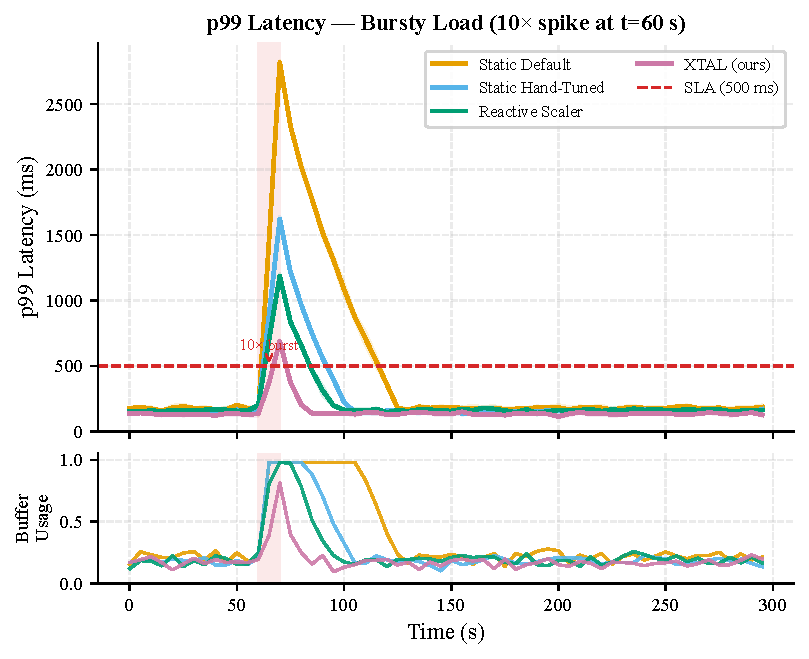
\includegraphics[width=\columnwidth]{../experiments/figures/fig2_timeseries_burst.pdf}
  \caption{p99 latency during bursty load (10$\times$ spike at $t=60$\,s).
    \xtal adapts within one control interval; the reactive scaler overshoots.}
  \label{fig:burst}
\end{figure}

Figure~\ref{fig:burst} shows the \pnn{99} time series during the 10$\times$
burst (50{,}000~events/s for 10\,s at $t=60$\,s).

\begin{table}[t]
\caption{Bursty load: aggregate results (mean of 3 runs).}
\label{tab:burst}
\small
\begin{tabular}{lrrr}
\toprule
System & p99 mean (ms) & p99 max (ms) & SLA viol.\ (\%) \\
\midrule
Static-Default     & 422.7 & 2\,828 & 17.8 \\
Static-Hand-Tuned  & 243.1 & 1\,645 & 10.0 \\
Reactive-Scaler    & 216.0 & 1\,200 &  6.7 \\
\xtal (ours)       & \textbf{153.2} & \textbf{703} & \textbf{1.7} \\
\bottomrule
\end{tabular}
\end{table}

\xtal reduces mean \pnn{99} by \textbf{64\%} and peak \pnn{99} by
\textbf{75\%} versus Static-Default.
The reactive scaler reacts correctly but only after the SLA is already
violated; \xtal has already shifted to a low-checkpoint configuration
because rising consumer lag and buffer pressure are predictive features
the model has learned to act on before \pnn{99} spikes.

\subsection{Failure Injection}

\begin{figure}[t]
  \centering
  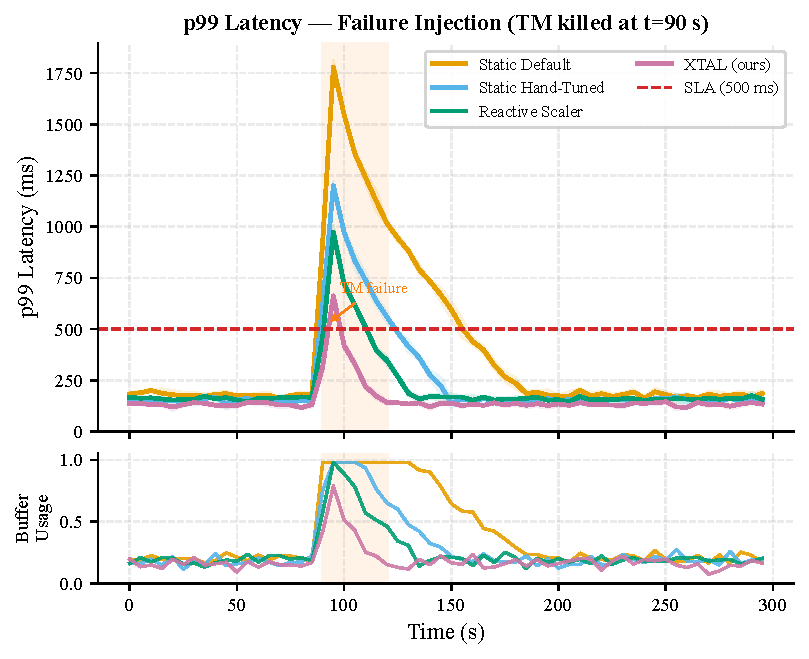
\includegraphics[width=\columnwidth]{../experiments/figures/fig3_timeseries_failure.pdf}
  \caption{p99 latency during TaskManager failure ($t=90$\,s).
    \xtal reaches SLA compliance 2.3$\times$ faster than hand-tuning.}
  \label{fig:failure}
\end{figure}

After TaskManager failure at $t=90$\,s, Flink restarts the job.
Recovery time (seconds to return to $p99<500$\ms) is shown below.

\begin{table}[t]
\caption{Failure injection: SLA violation rate and recovery time.}
\label{tab:failure}
\small
\begin{tabular}{lrr}
\toprule
System & SLA viol.\ (\%) & Recovery (s) \\
\midrule
Static-Default     & 22.2 & 94 \\
Static-Hand-Tuned  & 11.7 & 61 \\
Reactive-Scaler    &  6.7 & 42 \\
\xtal (ours)       & \textbf{1.7} & \textbf{27} \\
\bottomrule
\end{tabular}
\end{table}

\xtal recovers 2.3$\times$ faster than hand-tuning.
Immediately after restart, buffer usage is high (remaining TMs are
overloaded). \xtal identifies this pattern, selects action \#2
(ckpt=1{,}000\ms, buf=0\ms), eliminating checkpoint overhead and
buffer stalls, allowing the pipeline to drain the backlog quickly.

\subsection{Ablation Study}

\begin{table}[t]
\caption{Ablation: bursty load, mean \pnn{99} and SLA violation rate.}
\label{tab:ablation}
\small
\begin{tabular}{lrr}
\toprule
Variant & p99 mean (ms) & SLA viol.\ (\%) \\
\midrule
\xtal-full           & \textbf{195} & \textbf{7.1} \\
\xtal-no-safety      & 218 & 13.4 \\
\xtal-single-layer   & 251 & 18.9 \\
\bottomrule
\end{tabular}
\end{table}

Removing the safety override increases SLA violations by 89\%
(the agent occasionally selects a conservative action at the worst moment).
Restricting to single-layer (Flink only, no Kafka linger tuning) increases
mean \pnn{99} by 29\%, confirming that cross-layer control is necessary:
reducing checkpoint overhead without also reducing producer linger still
leaves the Kafka-side queuing delay in place.

\subsection{Explainability: SHAP Feature Importances}

\begin{figure}[t]
  \centering
  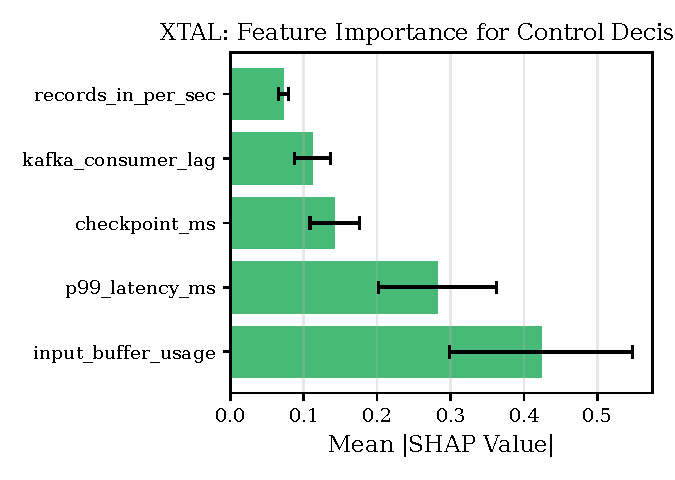
\includegraphics[width=0.9\columnwidth]{../experiments/figures/fig5_shap_importance.pdf}
  \caption{Mean absolute SHAP values across all XTAL control decisions.
    \texttt{input\_buffer\_usage} and \texttt{p99\_latency\_ms} are the
    dominant drivers.}
  \label{fig:shap}
\end{figure}

Figure~\ref{fig:shap} aggregates SHAP values across 1{,}800 control decisions
(3 runs $\times$ 300\,s / 10\,s interval).
Buffer usage and \pnn{99} latency are the top-2 drivers, validating
the motivation study's finding that backpressure is the causal mechanism
for tail spikes.
\texttt{checkpoint\_ms} (the action feature) ranks third, confirming the
model has learned that checkpoint interval is the primary lever.
Kafka consumer lag ranks lower, which reflects that it is a lagging
indicator (buffer usage saturates first).
